\documentclass[document.tex]{subfiles}
\begin{document}
\chapter{Result and Performance Analysis}

\section{Result}
\noindent For calculating the performance of our system, we applied 5-fold cross-validation. For calculating the accuracy of our system, we use Eq. \ref{eq:acc}.
\begin{equation}
	Accuracy = {T_c \over T_s}
	\label{eq:acc}
\end{equation}

Where $T_c$ is the number of problems for which our system
\textbf{PWPS} gives correct solution and $T_s$ is the number of total problems. Fig. \ref{fig:accvsalpha} shows the accuracy with respect to several values for $\alpha$ and $\beta$ in Eq.\ref{eq:main}. In horizontal axes the values of $\alpha$ and
in vertical axes it shows the accuracy (\%).
\begin{figure}[H]
	\begin{center}
	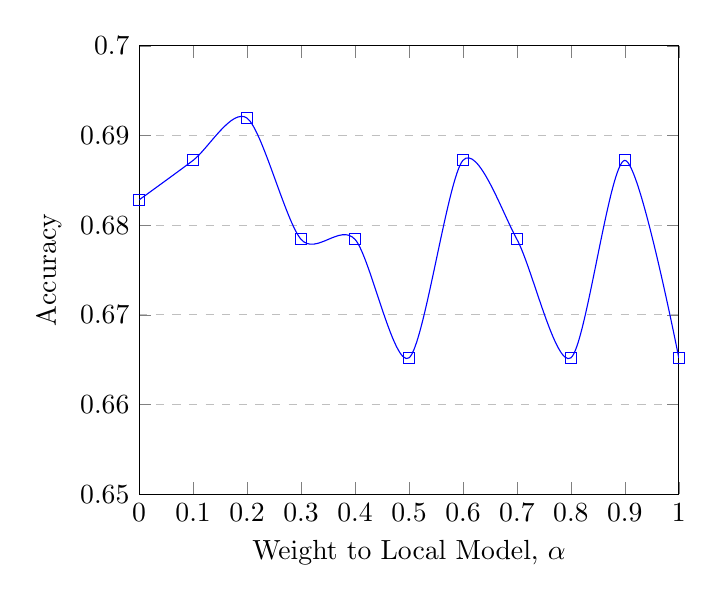
\begin{tikzpicture}
	\begin{axis}[
	%title={},
	xlabel={Weight to Local Model, $\alpha$ },
	ylabel={Accuracy},
	xmin=0, xmax=1,
	ymin=0.65, ymax=0.70,
	xtick={0.0, 0.1,0.2,0.3,0.4,0.5,0.6,0.7, 0.8, 0.9, 1.0},
	ytick={0.65, 0.66, 0.67, 0.68,0.69, 0.70},
	legend pos=north west,
	ymajorgrids=true,
	grid style=dashed,
	]
	
	\addplot[
	blue,
	mark=square,
	smooth,
	]
	coordinates {
		(0.0, 0.6828193832599119)
		(0.1, 0.6872246696035242)
		(0.2, 0.6919299559471366)
		(0.3, 0.6784140969162996)
		(0.4, 0.6784140969162996)
		(0.5, 0.6651982378854625)
		(0.6, 0.6872246696035242)
		(0.7, 0.6784140969162996)
		(0.8, 0.6651982378854625)
		(0.9, 0.6872246696035242)
		(1.0, 0.6651982378854625)
	};
	%		\legend{CuSO$_4\cdot$5H$_2$O}
	
	\end{axis}
	\end{tikzpicture}
	\end{center}
	\caption{Accuracy Versus $\alpha$}
	\label{fig:accvsalpha}
\end{figure}

In our dataset, a total number of problems is \textit{185}, and our system could solve problems \textit{128} correctly. Based on this, the accuracy of our system is \textbf{69.19\%}. Fig. \ref{fig:accvsalpha} show the accuracy for different values of $\alpha$. In reverse that is also for $\beta$. The values in horizontal axes represents the value for $\alpha$ and the values in vertical axes represents the accuracy based on that. We have seen that the accuracy sometimes increases and sometime decreased based on $\alpha$. We have changed the value of $\alpha$ by \textit{0.1} and for $\alpha=0.2$ where $\beta = 1 – 0.2 = 0.8$ is the optimal value for Eq. \ref{eq:main} and the accuracy is maximized.

\subsection{Comparison}
From Fig. \ref{fig:accvsalpha}, we can see that our system’s performance is high for $\alpha = 0.2$ and $\beta  = (1 – 0.2) = 0.8$.
\begin{table}[H]
	\caption{Comparison Between scoring based on equation of PWPS and ALGES}
	\begin{center}
		\begin{tabular}{|l|l|}
			\hline
			Equation of System & Accuracy (\%)\\
			\hline
			PWPS & \textbf{69.19}\\
			ALGES & 67.84\\
			\hline
		\end{tabular}
	\end{center}
	\label{tab:comp}
\end{table}


Table \ref{tab:comp} shows that the accuracy of \textbf{PWPS} is \textbf{69.19\%} which is better than the score using ALGES’s equation.

\subsection{Ablation Study}
In order to determine the effect of various components of our system on its overall performance, we perform the following ablations:
\subsubsection{No Local Model}
We test our system without a local model for generating the equations. Moreover, it is only based on Global Model. So, $\alpha = 0.0$ and $\beta = 1.0$. Without Local Model Eq. \ref{eq:main} is like below:
\begin{equation}
	p(t|p) = (\beta * G_{global}(t|p))
	\label{eq:Noloc}
\end{equation}
\subsubsection{No Global Model}
Here, we test our system without the global model for generating the equations which are based on the all local score of the equation. For $\alpha = 1.0$ and $\beta = 0.0$ equation without Global Model \ref{eq:main} is like below:
\begin{equation}
	p(t|p) = (\alpha * \prod_{t_i \in t} L_{local}(t_i | p) ) 
	\label{eq:noGlob}
\end{equation}

Table \ref{tab:ablation} shows the result of ablation study of our system. Accuracy of PWPS is better than the No Local Model and No Global Model system.
\begin{table}[H]
	\caption{Ablation Study of PWPS}
	\begin{center}
		\begin{tabular}{|l|l|}
			\hline
			Method & Accuracy (\%)\\
			\hline
			PWPS & \textbf{69.19}\\
			No Local Model & 68.28\\
			No Global Model & 66.52\\
			\hline
		\end{tabular}
	\end{center}
	\label{tab:ablation}
\end{table}
Table \ref{tab:ablation} shows the result of ablation study of our system. Accuracy of \textbf{PWPS} is better than the No Local Model and No Global Model system.
\section{Error Analysis}
Parsing errors cause a wrong grounding into the
designed representation. For example, the parser
treats ‘regular’ as a noun modified by the number
‘13’, leading our system to treat ‘regular’ as the entity of a Qset rather than ‘Coffee’. Despite the
improvements that come from PWPS , a portion of
errors are attributed to grounding and ordering issues. For instance, the system fails to correctly distinguish between the sets of wheels, and so does not get the movement-triggering container relationships right. Semantic limitations are another source of errors. For example, PWPS does not model the semantics of ‘three consecutive numbers’. 
\begin{table}[H]
	\caption{Error in PWPS}
	\begin{center}
		\begin{tabular}{|l|l|}
			\hline
			Error Type & Problem Text (\%)\\
			\hline
			Parsing Issues& Kira’s Cafe has regular coffee and decaffeinated coffee. This  \\
			&morning, the cafe served \underline{\textit{13} regular} coffees and \underline{\textit{39} decaffeinated}\\
			& coffees. What percentage of the coffees served were regular?\\
			\hline
			Grounding Issues & There are \underline{24 bicycles} and \underline{14 tricycles} in the storage at Danny’s\\
			& apartment building. Each bicycle has 2 wheels and each tricycle \\
			&has 3 wheels. What percentage of wheels are there in bicycle?\\
			\hline
		\end{tabular}
	\end{center}
	\label{tab:grounding}
\end{table}
Finally, \textbf{PWPS} is not able to infer quantities when they are not explicitly mentioned in the text. 

\end{document}
